\documentclass[a4paper,11pt]{article}
\usepackage[T1]{fontenc} 
\usepackage[dvips]{graphicx}
\usepackage{fancyhdr}
\pagestyle{fancy}
\lhead{BEARIFY - Requirements specification version 1.0}
\chead{}
\rhead{\thepage}
\lfoot{}
\cfoot{}
\rfoot{}
\begin{document}
 
\thispagestyle{empty}
\vspace*{2cm}
\begin{center}
{\LARGE BEARIFY REQUIREMENTS SPECIFICATION}

\vspace{1.5cm}

\begin{tabular}{|l|l|}							\hline
\multicolumn{2}{|c|}{\textbf{PROJECT INFORMATION}} 		\\	\hline
\textbf{Project Name:}		& Bearify \\ \hline
\textbf{Project Manager:}	& Erik Gregg \\	\hline
\end{tabular}

\vspace{2cm}

\begin{tabular}{|l|l|}							\hline
 \multicolumn{2}{|c|}{\textbf{DOCUMENT INFORMATION}}  \\	\hline
\textbf{Subject:}		& Requirements specification	\\	\hline
\textbf{Authors:}		& Timo Ahonen			\\	\hline
\textbf{Keywords:}		&				\\	\hline
\textbf{Comments:}		&				\\	\hline
\textbf{Creation date:}		& 25.1.2002 			\\	\hline
\textbf{Revision date:}		& 2.2.2002			\\	\hline
\textbf{Document Status:}	& [ ] Draft			\\	\hline
				& [ ] Proposal			\\	\hline
				& [X] Inspected \& approved	\\	\hline
\textbf{Revision History:}	& 25.1.2002 Version 0.1 Original draft by TA \\	\hline
				& 27.1.2002 Version 0.2 Improved draft by TA  \\
				& after discussion with Sauli Kivikunnas		\\ 	\hline
				& 28.1.2002 Version 1.0 Proposal for \\
				& inspection  meeting by TA  \\ \hline	
				& 2.2.2002 Version 1.1 Corrected after  \\
				& inspection meeting by TA\\ 	\hline
				& 6.2.2002 Version 1.1 Correnctions \\
				& approved by TR  \\ 	\hline
				& { } 				\\ 	\hline
				& { } 				\\ 	\hline
\end{tabular}
\end{center}
\newpage

\tableofcontents
\newpage

\section{Introduction}

\subsection{Purpose}

The purpose of this document is to specify the requirements of the Dynamic Time Warping Trend Analysis Tool,
which will be created within the DTREND-project. The supplier in the project is the DTREND group and the customer 
is VTT Electronics.

This software project is intended to fulfill the requirements of the Advanced Software Engineering Project course 
(52479S) of University of Oulu.

\subsection{Scope}

The aim of the project is to create a pattern recognition tool for process monitoring and diagnostics to be used in
VTT's research projects.

The customer may use some of the components created in the DTREND project in its own software projects. 
However, the DTREND project is completely independent of these other projects. 

\subsection{Acronyms and symbols}
\begin{tabular}{ll}
DLL 	& Dynamic Link Library. \\
DTW	& Dynamic Time Warping. \\
GUI & Graphical User Interface \\
\\
$S$	& The observation vector. \\
$s_i$	& An element of the observation vector S. \\
$n$	& Length (dimension) of the observation vector.\\
$T$	& The template vector. \\
$t_j$	& An element of the template vector T. \\
$m$	& Length of the template vector. \\
$W$	& The warping path vector. \\
$w_k=(i_k,j_k)$	& An element of the warping path vector W. \\
$p$	& Length of the warping path vector. \\
$K$	& Length of the warping path. \\
$k$	& An unique index number of a template.\\
$A$	& A set of all allowable warping paths. \\
$\omega$	& The warping window width. \\
$\delta$	& Warping path start and end point offset. \\
\end{tabular}

\subsection{References}

$[1]$ IEEE 830--1998 Standard \\
\\
$[2]$ Berndt, D.J. \& Clifford, J. 1996. Finding patterns in time series: A dynamic programming approach. 
In: Fayyad, U.M., Piatetsky-Shapiro, G., Smyth, P. \& Uthurusamy R. (eds.) Advances in Knowledge Discovery
and Data Mining. Menlo Park, AAAI Press / The MIT Press. P. 229-248. \\
\\
$[3]$ Keogh, Eamonn J. \& Pazzani, Michael J. 2001. Derivative Dynamic Time Warping. First {SIAM} International 
Conference on Data Mining {(SDM'2001)}, April 5-7, Chicago, {IL}. {USA}. \\
\\
$[4]$ Paulus, D. W. R. \& Hornegger, J. 1998. Applied Pattern Recognition: A Practical Introduction to Image and
Speech Processing in C++. Wiesbaden, Verlag Vieweg. 405 p. \\
\\
$[5]$ Synthetic Control Chart Time Series, University of California, Irvine, {USA}. Last update 14.6.1998. Referenced
on 27.1.2002. \\
<http://kdd.ics.uc.edu/databases/synthetic\_control/\\synthetic\_control.html> \\
\\
$[6]$ Dynamic Time Warping Digit Recognizer, Institution for Signal and Information Processing, Missisippi State University, 
{USA}. Last update 18.1.2002. Referenced on 27.1.2002. \\ 
<http://www.isip.msstate.edu/projects/speech/software/demonstrations/\\applets/util/dynamic\_time\_warping/current/index.html> \\
\\
$[7]$ Intel Recognition Primitives Library. Referenced on 27.1.2002. \\ 
<http://developer.intel.com/software/products/perflib/rpl/index.htm>

\subsection{Overview}
The rest of this document is divided into four parts. Section 2 contains a general introduction to the functions of the
DTREND tool. Specific descriptions of the product functions are in section 3. The last two sections contain some general
requirements concerning the whole project.
 
This document complies with IEEE Recommended Practice for Software Requirements Specifications $[1]$.

\section{General description}

\subsection{Project perspective}

The goal of the DTREND project is to create a research tool which implements the Dynamic Time Warping algorithm. 
The tool will be used in research projects of VTT Electronics. These research projects are concerned with process 
monitoring and diagnostics. The main goal of the DTREND tool is recognition of patterns in measurement time series. 

The most important characteristic of the DTW algorithm and DTREND tool is the ability to cope with variation on the
time axis, i.e. some parts of the signal may be shrunken whereas other parts may be stretched.

\begin{figure} 
\begin{center} 
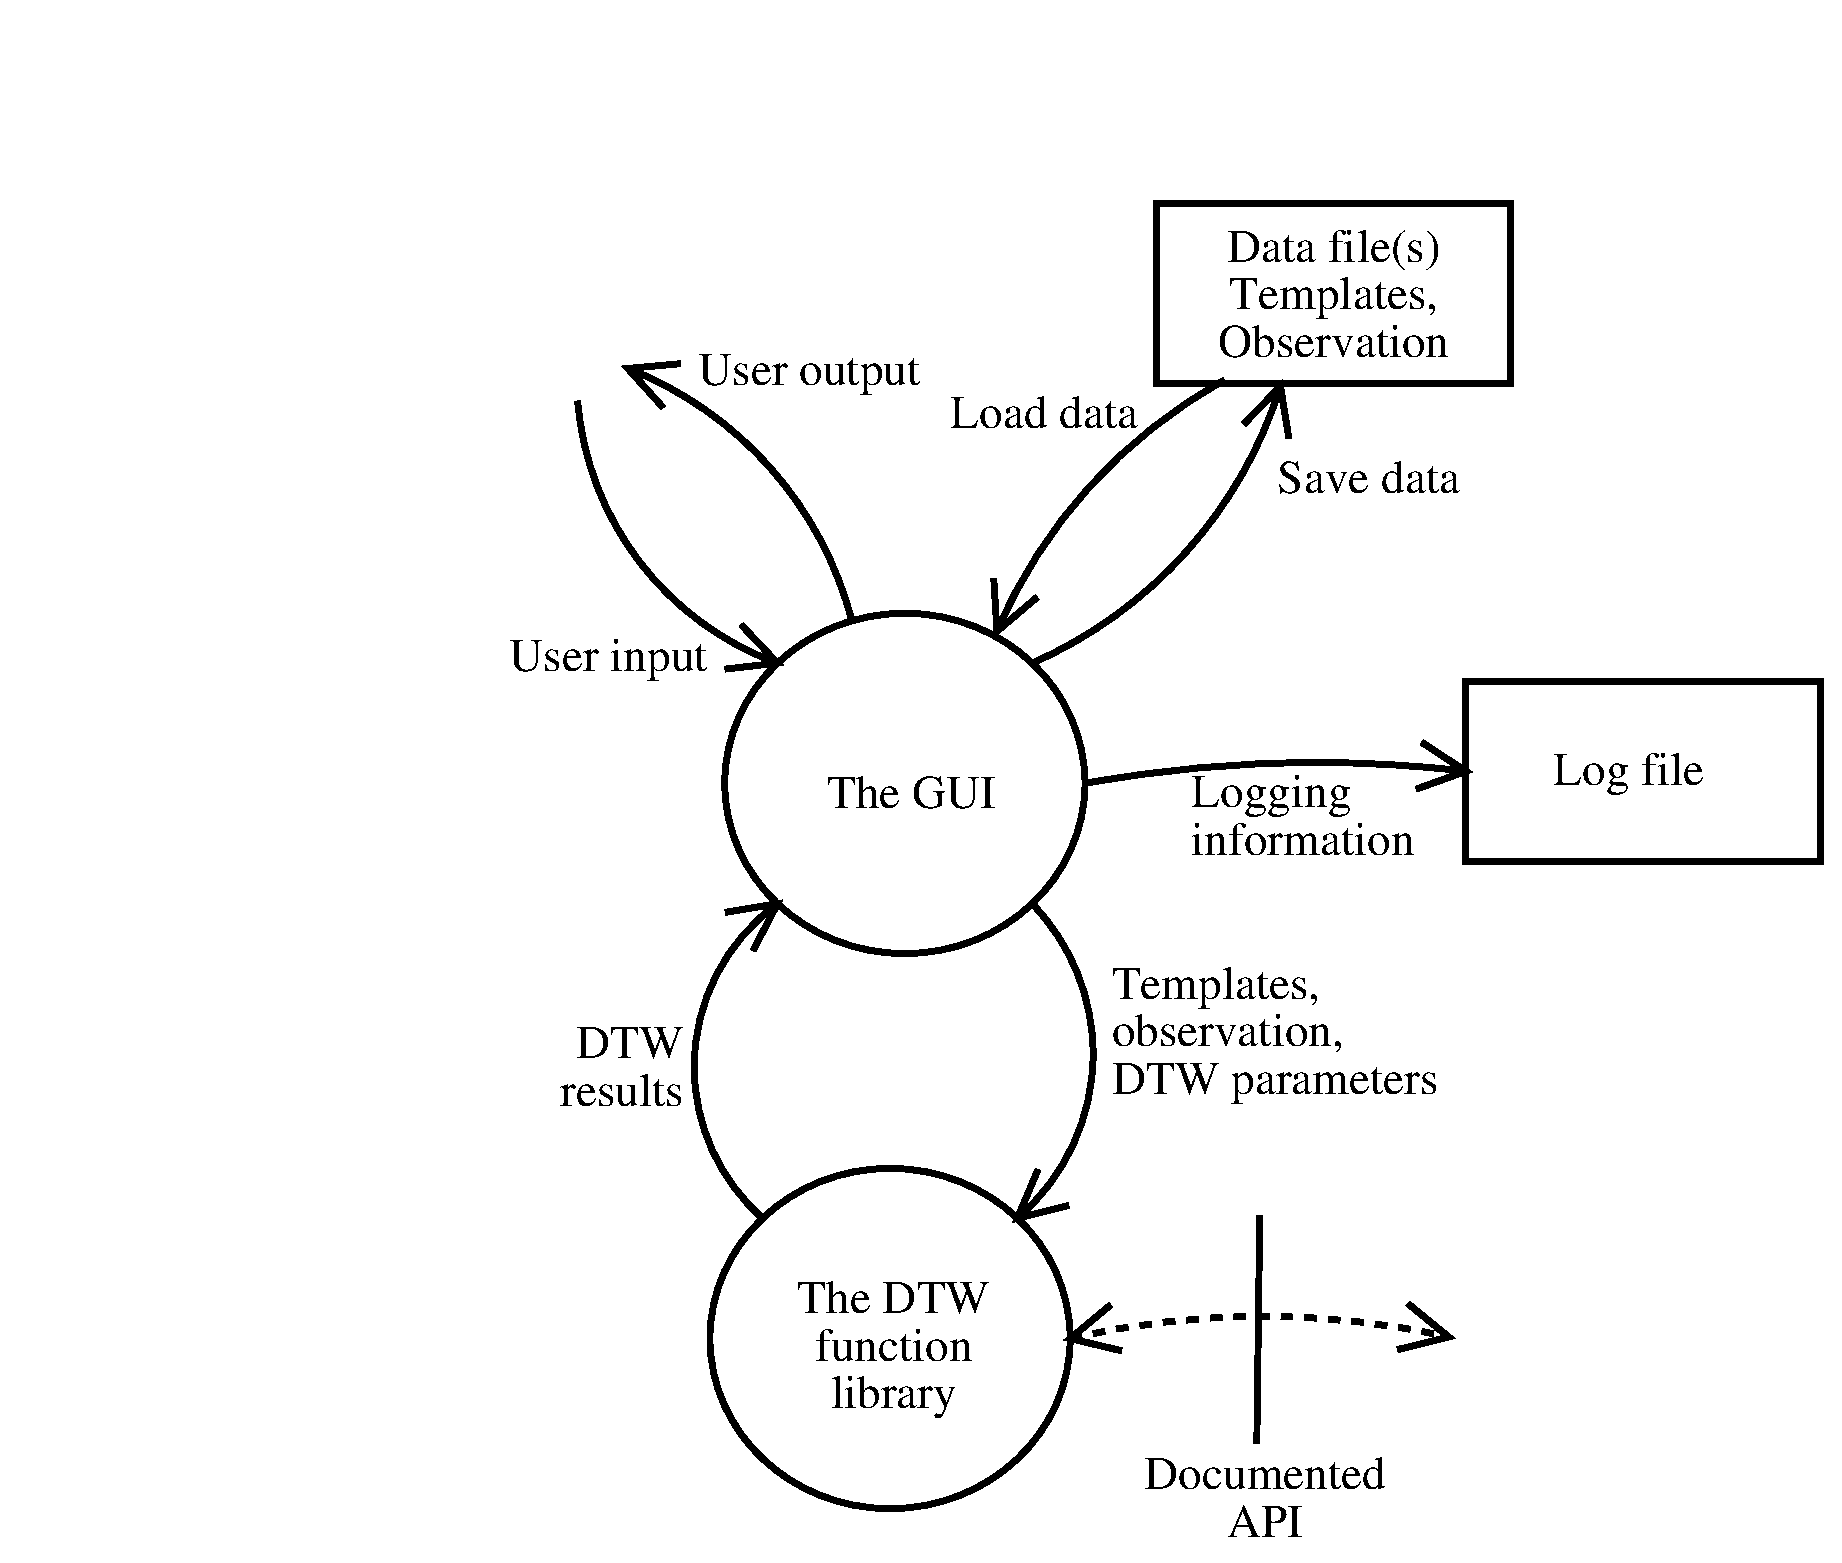
\includegraphics[width=0.7\textwidth]{srs_components.eps}
\caption{Parts of the DTREND software} 
\label{fig:components}
\end{center} 
\end{figure}

The DTREND tool must be divided into two parts: A function library, which implements the DTW algorithm and a 
executable which utilizes the function library. The executable part is called the GUI part in this document, even though
strictly speaking, not all of its functions are those of a GUI. The parts of the software are visualized in Figure 
\ref{fig:components}.

\subsection{Product functions}

\subsubsection{Use cases}
\begin{enumerate}
\item Load records from a text file.
\item Pick part(s) of a record to be used as templates or as an observation.
\item Name the templates and the observation.
\item Save the templates to a text file.
\item Save the observation to a text file.
\item Load an observation from a text file.
\item Load templates from a text file.
\item Choose the parameters of the DTW algorithm. These include
\begin{enumerate}
\item Global constraints
\item Local constraints
\item How the distance between two points is determined
\end{enumerate}
\item Compare the observation against all templates using the DTW algorithm and announce, which template matches best
and the distance between the observation and the template found.
\item Compare the observation against a chosen template and show the distance between them.
\item Show the warping grid and the warping path of the last run. Show also the lengths of the axes (i.e. the length
of the template and the observation).
\item Draw plots of the (best-fit) template and the observation of the last DTW run.
\item Save the parameters and the results of the run to a log file.
\end{enumerate}

\subsubsection{The DTW algorithm}
\label{sec:dtw}
The DTW algorithm is so essential part of the software that it will be discussed here briefly. More thorough descriptions
can be found in the references $[2]$, $[3]$ and $[4]$.

We have two time series, $S$ and $T$. Let $d(i,j)$ be the distance between points $s_i$ and $t_i$. Now we try to find
such path $W$ in the $i \times j$ matrix that minimizes the quotient
\begin{equation}
\frac{\sum_{k=1}^p d(w_k)}{K} = \frac{\sum_{k=1}^p d(i_k,j_k)}{K}
\end{equation}
where K is the length of the path. Now we have
\begin{equation}
DTW(S,T)=\min_W \frac{\sum_{k=1}^p d(w_k)}{K}
\end{equation}

We restrict the algorithm by a local constraint so that the path may go from point $(i_k,j_k)$ to 
point $(i_k+1,j_k)$, $(i_k+1,j_k+1)$ or $(i_k,j_k+1)$ , i.e. we set continuity and monotonicity requiremnts.

The set of allowable paths may be restricted with parameters discussed in section \ref{sec:paramreq}. When parameter $P_1$
restricts the paths to set $A_1$ and simultaneously parameter $P_2$ to set $A_2$, the total set of allowable paths 
is the intersection of these two sets, i.e.
\begin{equation}
A=A_1 \cap A_2
\end{equation} 

\subsubsection{Software functions}
The software functions are listed here. A complete description of these functions is in section \ref{sec:funcreq}

\noindent DLL library functions
\begin{itemize}
\item \emph{D-01}: Load template
\item \emph{D-02}: Delete template
\item \emph{D-03}: One to all comparison
\item \emph{D-04}: One to one comparison
\item \emph{D-05}: Return template 
\end{itemize} 

\noindent GUI functions
\begin{itemize}
\item \emph{G-01}: Load data set 
\item \emph{G-02}: Select data
\item \emph{G-03}: Save selection
\item \emph{G-04}: Save vector to file
\item \emph{G-05}: Load vector from file
\item \emph{G-06}: Delete template from GUI
\item \emph{G-07}: Select DTW parameters
\item \emph{G-08}: Compare to all
\item \emph{G-09}: Compare to one
\item \emph{G-10}: Save results to log
\item \emph{G-11}: Show plots
\end{itemize}

\noindent DTW parameters
\begin{itemize}
\item \emph{P-01}: Distance metrics
\item \emph{P-02}: Warping window
\item \emph{P-03}: Slope constraint
\item \emph{P-04}: Start and end point offset
\end{itemize}


\subsection{User characteristics}
First user group of the tool is research personnel, who are familiar with the DTW algorithm. This user group needs 
especially a logging feature.

Another user group is research personnel who use the tool in learning the method. For this user group, the tool must contain 
a clear GUI with possibility to plot the observation and template vectors and the warping path on the screen.

The third user group which has to be considered during the software project are other software engineers who do further 
development of the tool. To make further development as easy as possible, the software must be well documented.

\subsection{General constraints}
The tool will be run on a PC workstation running Microsoft Windows NT.

The DTW algorithm must be implemented in a Windows DLL library. The library must be well documented, because the
customer may use it in its own projects. 

The tool is stand-alone, i.e. there is no need for network functionality.

The amount of work reserved for the project is three man months.

The product must be ready and tested by the 15th March 2002.

\subsection{Assumptions and dependencies}

The non-free tools (eg. Microsoft Visual C++) needed within the project will be provided by the customer. 


\section{Structural overview and specific requirements}

\subsection{Functional requirements} 
\label{sec:funcreq}

In this section, the DLL library and the GUI are handled separately. The GUI must use the functions provided by 
the DLL. The requirements concerning the parameters of the DTW are also in a separate section.

The requirements are divided into three classes:
\begin{itemize}
\item Essential: Abscence or malfunction of these functions makes the software unusable, in which case the project will not be accepted. 
\item Conditional: These functions are not absolutely necessary, but leaving them out decreases significantly the value of the
product.
\item Optional: These functions may or may not be worthwhile and the supplier may propose leaving them out at design
or implementation stage.
\end{itemize}

A more thorough description of these three classes can be found in reference $[1]$.

\subsubsection{The DLL library}

\noindent \emph{Functional requirement D-01: Load template (Essential)}
\begin{itemize}
\item Introduction:

The DLL must contain a function to load templates into it.

\item Input:

A vector $T$ of floating point values and the length of the vector.

\item Processing:

The DLL copies the values into its internal data structures to be used by functions \emph{D-03} and \emph{D-04}.

\item Output:

A unique index number $k$ of the saved template.
\end{itemize}

\noindent \emph{Functional requirement D-02: Delete template (Conditional)}
\begin{itemize}
\item Introduction:

The DLL must contain a function to delete templates from its data structures.
\item Input:

Index number $k_d$ of the template to be deleted
\item Processing:

The DLL deletes the template in question from its data structures.
\item Output:

None
\end{itemize}


\noindent \emph{Functional requirement D-03: One to all comparison (Conditional)}
\begin{itemize}
\item Introduction:

The DLL must contain a function to compare a given observation against all templates.
\item Input:

\begin{enumerate}
\item A vector $S$ of single-precision floating point values containing the observation
\item The length of the vector $S$
\item A structure containing the parameters for the algorithm. These parameters are discussed in section \ref{sec:paramreq}
\end{enumerate}

\item Processing:

The DLL runs the DTW algorithm between the observation and every template that the user has entered earlier.
\item Output:

A vector of vectors, which contain two values:
\begin{enumerate}
\item Index number of a template
\item The calculated DTW difference between the observation and the template in question
\end{enumerate}
\end{itemize}

\noindent \emph{Functional requirement D-04: One to on comparison (Essential)} 

\begin{itemize}
\item Introduction:

The DLL must contain a function to compare a given observation against one specific template.
\item Input:

\begin{enumerate}
\item A vector $S$ of single-precision floating point values containing the observation
\item The length of the vector $S$
\item A structure containing the parameters for the algorithm. These parameters are discussed in chapter \ref{sec:paramreq}
\item Index number of the template that the observation is compared against
\end{enumerate}

\item Processing:

The DLL compares the observation against the selected template using the DTW algorithm with selected parameters.
\item Output:

\begin{enumerate}
\item The DTW difference between the observation and the template
\item A vector $W$ containing the best-fit warping path. The vector consists of $(i,j)$-pairs that define
the path.
\item Length of vector $W$
\end{enumerate}
\end{itemize}


\noindent \emph{Functional requirement D-05: Return template (Essential)}
\begin{itemize}
\item Introduction:

The DLL must contain a function to return a template that has been stored in its data structures.
\item Input:

The index $k$ of the template to be returned.
\item Processing:

The DLL returns the template in question.
\item Output:

\begin{enumerate}
\item The requested template, $T_k$.
\item Length of $T_k$.
\end{enumerate}
\end{itemize}

\subsubsection{Functional requirements of the GUI}
\label{sec:guireq}


\noindent \emph{Functional requirement G-01: Load data set (Conditional)}
\begin{itemize}
\item Introduction:

The user must be able to load a data set from a text file.
\item Input:

The file is selected with a file selection dialog.
\item Processing:

The GUI shows the file selection dialog. When user has selected the file, GUI opens the file in a data selection
view described in requirement \emph{G-02}. The file format is described in section \ref{sec:datafile}. 
\item Output:

If the file format is invalid, the GUI shows an error message and returns to main view. Otherwise, the GUI opens
the data selection view.
\end{itemize}


\noindent \emph{Functional requirement G-02: Select data (Conditional)}
\begin{itemize}
\item Introduction:

There must be a data selection view, which can be used to select parts of the data set. See figure \ref{fig:selview}. Note
that the figure is intended only to clarify, what elements the selection view must contain.

\begin{figure} 
\begin{center} 
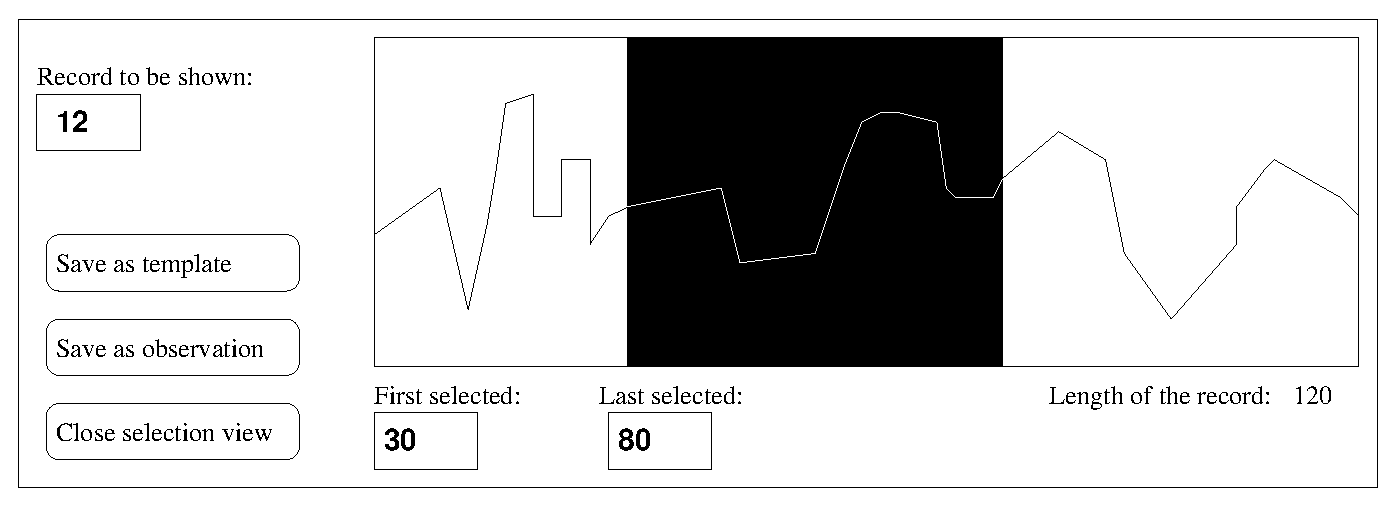
\includegraphics[width=0.8\textwidth]{srs_selview.eps}
\caption{Contents of the data selection view} 
\label{fig:selview}
\end{center} 
\end{figure}

\item Input:

The file opened at stage \emph{G-01}. 

The selection view itself must contain following user inputs:
\begin{itemize}
\item Which record of the data set is to be shown
\item Select a part of the record plot by painting
\item Select a part of the record plot by entering the indexes of the first and last element to be selected.
\end{itemize}
\item Processing:

When user selects the record to be shown, the chosen record must be read from the data set file and shown as a 
trend plot in the view. When user selects a part of the record by painting, the ``first element'' and ``last 
element'' fields are updated respectively and vice versa. The selected area is marked in reverse colours. 
When user chooses to save the selected part as a template or as an observation, a vector containing the values
inside the selection is passed along.
\item Output:

\begin{itemize}
\item A plot of the chosen record and the record length.
\item A vector containing the elements inside the selection and the length of the vector.
\end{itemize}
\end{itemize}


\noindent \emph{Functional requirement G-03: Save selection (Conditional)}
\begin{itemize}
\item Introduction:

The user must be able to save the selected part as a template or as an observation. 
\item Input:

A vector from \emph{G-02} containing the values to be saved and the length of the vector and following user inputs:
\begin{itemize}
\item Is the selection intended to be saved as a template or as an observation
\item A name for the template / observation 
\end{itemize}
\item Processing:

When user chooses to save the selected part, he is asked to name it. Then the selection is saved as a template
or as an observation. There may be only one observation in the memory at a time, so if the selection is saved as
an observation, the previous observation is erased.

\item Output:

None
\end{itemize}


\noindent \emph{Functional requirement G-04: Save vector to file (Conditional)}
\begin{itemize}
\item Introduction:

The user must be able to save the observation or the templates in memory to a text file. 
\item Input:
\begin{itemize}
\item Which data is to be saved: the observation or the templates
\item Name of the file
\item If the file exists, the user is asked whether to overwrite the file
\end{itemize}

\item Processing:

The user is shown a file selection dialog, using which he/she may choose, which file the information is saved to.
If the file exists, the user is asked whether to overwrite it. If the user selects not to overwrite the file, the
file name is asked again. There is no possibility to apped to files. After the file has been selected, the observation
or templates including the names given to them are saved to the file. The exact file format will be determined at design
stage.
\item Output:
\begin{itemize}
\item A message that the saving has succeeded or an error message.
\item The file containing the observation or the templates and their names
\end{itemize}

\end{itemize}


\noindent \emph{Functional requirement G-05: Load vector from file (Essential)}
\begin{itemize}
\item Introduction:

The user must be able to load templates and an observation directly from a text file.
\item Input:
\begin{itemize}
\item Which data is to be loaded: the observation or the templates
\item Name of the file
\end{itemize}

\item Processing:

The user is shown a file selection dialog. The selected file is opened and the data (name of the template/observation and
the values) is read into memory. The exact file format will be determined at design stage. If the user loads an observation, the
previous observation is erased. If the the user loads templates, they are added to the template list.
\item Output:
\begin{itemize}
\item A message to user that the loading has succeeded or an error message.
\item A list of vectors containg the loaded templates or observation
\end{itemize}

\end{itemize}


\noindent \emph{Functional requirement G-06: Delete template from GUI (Conditional)}
\begin{itemize}
\item Introduction:

The user must be able to delete templates from the memory (one at a time or all).
\item Input:
\begin{itemize}
\item Whether to delete one or all of the templates
\item The template to be selected 
\end{itemize}

\item Processing:

The programs deletes the selected templates from the memory.
\item Output:

None
\end{itemize}


\noindent \emph{Functional requirement G-07: Select DTW Parameters (Essential)}
\begin{itemize}
\item Introduction:

The user must be able to select the parameters of the DTW algorithm
\item Input:

The chosen parameters
\item Processing:

The parameters of the algorithm are described in section \ref{sec:paramreq}
\item Output:

None
\end{itemize}




\noindent \emph{Functional requirement G-08: Compare to all (Conditional)}
\begin{itemize}
\item Introduction:

The user must be able to compare the observation against all templates in memory.
\item Input:

None
\item Processing:

The program compares the observation against all templates in memory using the DTW algorithm with parameters chosen in
\emph{G-07}. 

\item Output:

\begin{itemize}
\item Name of the best-fitting template and the calculated DTW distance
\item A plot of the observation and the template and the warping path (see \emph{G-11})
\end{itemize}
\end{itemize}


\noindent \emph{Functional requirement G-09: Compare to one (Essential)}
\begin{itemize}
\item Introduction:

The user must be able to select one of the templates and run the DTW algorithm against it.
\item Input:
 
The selected template.
\item Processing:

The observation is compared against the chosen template with the DTW algorithm using the parameters selected in
\emph{G-07}.
\item Output:

\begin{itemize}
\item Name of the selected template and the calculated DTW distance
\item A plot of the observation and the template and the warping path (see \emph{G-11})
\end{itemize}
\end{itemize}


\noindent \emph{Functional requirement G-10: Save results to log (Conditional)}
\begin{itemize}
\item Introduction:

The user must be able to save the results of the last run to a log file.  
\item Input:

The results of the run and the name of the log file as user input.
\item Processing:

The user is shown a file selection dialog. If the user chooses a file that exists already, the user is asked whether
the file should be rewritten. There is no possibility to append to a file. The results are saved to the chosen file.
\item Output:
The thing listed here are the minimum requirements, i.e. also other things may be saved to the log file. 
\begin{enumerate}
\item If the last run was of type \emph{G-08}:
\begin{itemize}
\item Date and time
\item The algorithm parameters
\item Name of the observation
\item Name of every template in memory and the DTW distance between the template and the observation. The templates must
be in ascending order by the DTW distance.
\item Ordered list of points $w_k$ of the warping path of the best-fit template.
\end{itemize}

\item If the last run was of type \emph{G-09}:
\begin{itemize}
\item Date and time
\item The algorithm parameters
\item Name of the observation
\item Name of the template and the DTW distance between the observation and the template
\item Ordered list of points $w_k$ of the warping path.
\end{itemize}
\end{enumerate}

\end{itemize}


\noindent \emph{Functional requirement G-11: Show plots (Essential)}
\begin{itemize}
\item Introduction:

The observation, best-fit template, the warping path and the warping window must be visible in the GUI 
(see Figure \ref{fig:teobgrid}).
\begin{figure} 
\begin{center} 
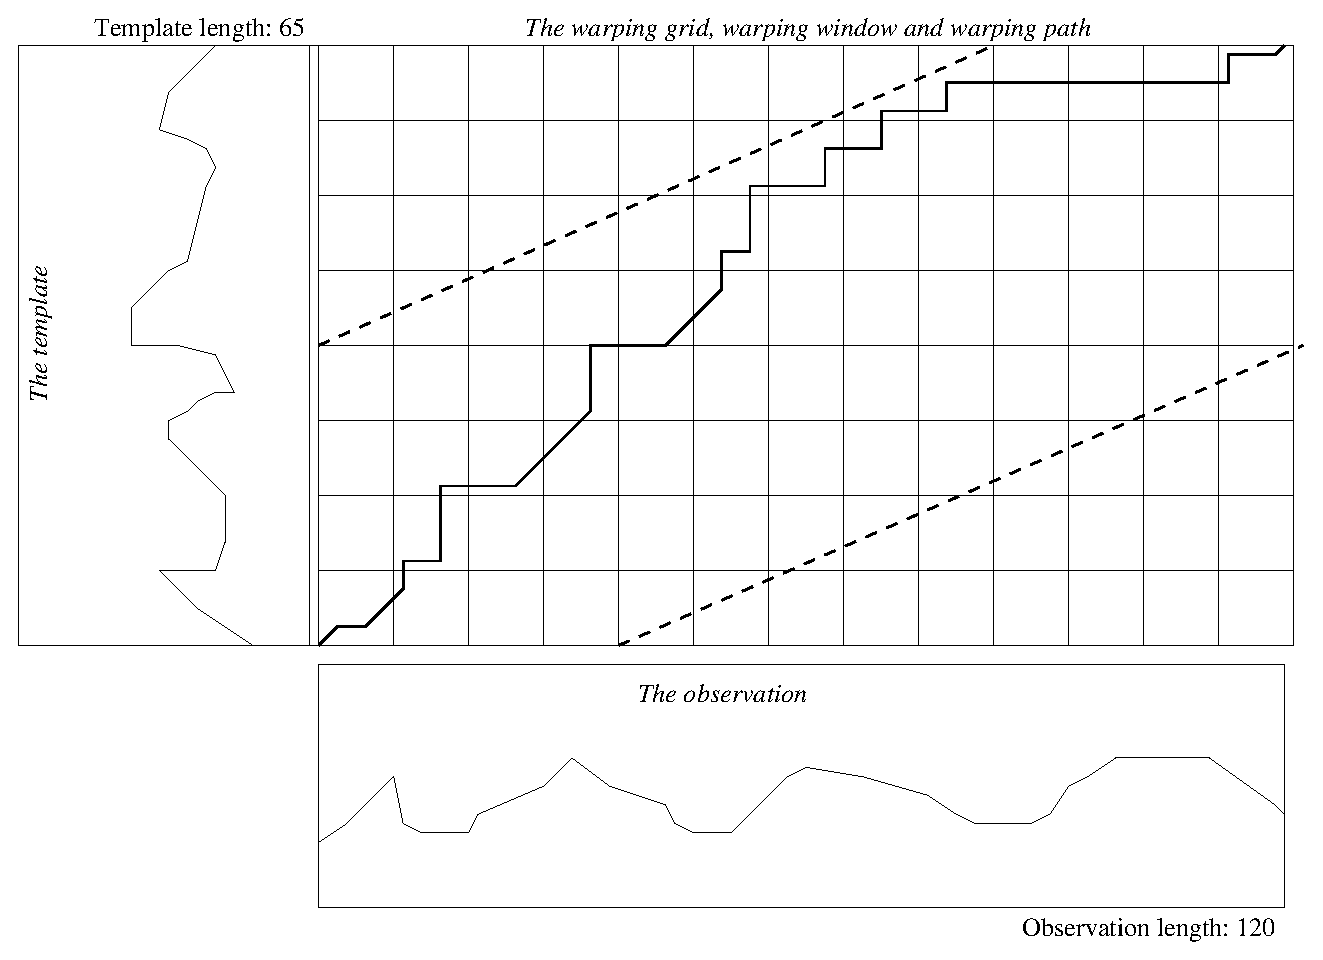
\includegraphics[width=0.8\textwidth]{srs_teobgrid.eps}
\caption{The template, observation, warping window and warping path} 
\label{fig:teobgrid}
\end{center} 
\end{figure}

\item Input:

The observation, template and warping path vectors and the warping window width $\omega$.
\item Processing:

The GUI draws plots of the vectors.
\item Output:

The plots and axis lengths as in Figure \ref{fig:teobgrid}. The observation is under the path and the template is on the left of
the path.
\end{itemize}

\subsubsection{Requirements concerning the parameters of the DTW algorithm}
\label{sec:paramreq}


\noindent \emph{Algorithm parameter requirement P-01: Distance metrics (Essential)}
\begin{itemize}
\item Introduction:

Two types of distance metrics must be supported: Euclidian and derivative metrics. The interfaces
must be designed so that it is easy to add support for other metrics at a later time.

\item A closer view:

See $[3]$.
\begin{enumerate}
\item Euclidian distance metrics:
\begin{equation}
d(i,j)=(s_i-t_j)^2
\end{equation}
\item Derivative distance metrics:
\begin{equation}
d(i,j)=(D_x[s_i]-D_x[t_j])^2,
\end{equation}
where $D_x[t_j]$ is an estimate of the derivative of $t_j$:
\begin{equation}
D_x[t_j]=\frac{(t_j-t_{j-1})+((t_{j+1}-t_{j-1})/2)}{2},
\end{equation}
when $2 \leq j \leq m-1$. The estimates for first and last elements of the sequece are defined followingly:
\begin{equation}
\begin{array}{rcl}
D_x[t_1] &=& D_x[t_2] \\
D_x[t_m] &=& D_x[t_{m-1}]
\end{array}
\end{equation}
\end{enumerate}

\end{itemize}




\noindent \emph{Algorithm parameter requirement P-02: Warping window (Essential)}
\begin{itemize}
\item Introduction:

The algorithm must be able to constrain the warping path inside a warping window. It must be possible
to change the size of the window.

\item A closer view:

See $[2]$, page 234. The warping path may contain only such points 
$w_k=(i_k,j_k)$ for which 
\begin{equation}
|i_k-j_k| \leq \omega
\end{equation}

The value of $\omega$ must be passed as a parameter to the algorithm.
\end{itemize}


\noindent \emph{Algorithm parameter requirement P-03: Slope constraint (Essential)}
\begin{itemize}
\item Introduction:

The algorithm must support only the slope constraint mentioned in chapter \ref{sec:dtw}. It must be possible
to add other slope constraints at a later time.

\item A closer view:

The warping path may go from point $(i_k,j_k)$ to point $(i_k+1,j_k)$, $(i_k+1,j_k+1)$ or $(i_k,j_k+1)$.
The interfaces must be designed so, that it is possible to implement other slope constraints (eg. 
Itakura slope constraint, see $[1]$).
\end{itemize}


\noindent \emph{Algorithm parameter requirement P-04: Start and end point offset (Conditional)}
\begin{itemize}
\item Introduction:

The algorithm must allow using fixed start and end points or a certain offset at the start and end points 
of the warping path. Fixed points are used by default.
\item A closer view:
\begin{enumerate}
\item Fixed points:

\begin{equation}
\begin{array}{rcl}
i_1 &=& 1 \\
j_1 &=& 1 \\ 
i_p &=& n \\
j_p &=& m . 
\end{array}
\end{equation}

\item Slightly relaxed points:
\begin{equation}
\begin{array}{rcccl}
1 &\leq& i_1 &\leq& 1+\delta \\
1 &\leq& j_1 &\leq& 1+\delta \\
n-\delta &\leq& i_p &\leq& n \\
m-\delta &\leq& j_p &\leq& m \\
\end{array}
\end{equation}
The value of $\delta$ must be passed as a parameter to the algorithm.
\end{enumerate}
\end{itemize}

\subsubsection{Dependencies between the functional requirements}
The following table shows how the requirements depend on other requirements, i.e. which requirements have to be completed
in order to complete next requirement.

\begin{tabular}{|l|l|}							\hline
\textbf{Requirement}					& \textbf{Depends on} 	  \\ \hline
\emph{D-01}			& -					  					\\ \hline
\emph{D-02}			& \emph{D-01}		  						\\ \hline
\emph{D-03}			& \emph{D-01, P-01, P-02, P-03}	\\ \hline
\emph{D-04}			& \emph{D-01, P-01, P-02, P-03}	\\ \hline
\emph{D-05}			& \emph{D-01}		  						\\ \hline
\emph{G-01}			& -					 						\\ \hline
\emph{G-02}			& \emph{G-01}		  						\\ \hline
\emph{G-03}			& \emph{G-02, D-01}		  				\\ \hline
\emph{G-04	}			& \emph{G-03, D-05}		  				\\ \hline
\emph{G-05}			& \emph{D-01}		  						\\ \hline
\emph{G-06}			& \emph{D-02}		  						\\ \hline
\emph{G-07}			& -					  						\\ \hline
\emph{G-08}			& \emph{D-03}		 						\\ \hline
\emph{G-09}			& \emph{D-04}		  						\\ \hline
\emph{G-10}			& \emph{D-05} and \emph{G-08} or \emph{G-09}		  		\\ \hline
\emph{G-11}			& \emph{G-08} or \emph{G-09}				\\ \hline
\emph{P-01}			& -				  							\\ \hline
\emph{P-02}			& -				  							\\ \hline
\emph{P-03}			& -				  							\\ \hline
\emph{P-04}			& -				  							\\ \hline
\end{tabular}


\subsection{External interface requirements}

\subsubsection{The data set file}
\label{sec:datafile}
The data set file is pure ASCII text file. One row contains one record. There is at least one row in the file.

A record contains at least three positive or negative decimal numbers separated with one or more spaces. The values 
are consecutive in time, and there is no time stamps for the values. A dot is used as a decimal separator. A number doesn't 
necessarily have to contain a decimal separator.

Particularly, the program must be able to read the data file in reference $[5]$.

\subsubsection{The graphical user interface}
The graphical user interface must contain only subdued colours. The GUI must contain VTT's logo.

\subsection{Performance requirements}
Since the DTREND tool is intended to be a research tool, there are quite few specific requirements. Some typical values for
vector lengths are stated here.

Typical length of observation and template vectors is less than 60. Yet, the data structures must be designed so that there is no
absolute limit for the lengths (apart from the physical memory available).

Typical number of templates in memory at a time is 12 and the maximum number is 40. Use of dynamic data structures is advisable
here, too.

The maximum running time for one to one comparison (\emph{G-09}) with vectors of length 60 is 10 seconds.

\subsection{Design constraints}
The DLL library must be implemented in C++ and the GUI in Java.

\section{General requirements}

\subsection{Security requirements}

There are no specific security requirements.

\subsection{Reliability requirements}
\label{sec:reliability}
The GUI must handle following exceptions and show a message describing the error:
\begin{itemize}
\item Invalid user input (eg. text instead of a number)
\item File not found
\item No access to a file
\item Invalid file format
\end{itemize}

\subsection{Maintainability requirements}

It is possible that the customer continues developing the software. It is important to pay attention to this during
the software design and implementation.

The DTREND project group is not responsible for maintaining the software after the project.

\subsection{Portability requirements}

Because of the use of the DLL technology the software is rather tightly bound to Microsoft Windows environment. There is
no need to consider portability in design or implementation.

\subsection{Installation requirements}
No installation program is needed.

\subsection{Administration handling}
Default configuration may be coded into the software. There is no need for further configuration handling

\subsection{Diagnostic requirements}
Apart from the error messages mentioned in section \ref{sec:reliability} there are no specific diagnostic requirements. 
The log file mentioned in section \ref{sec:guireq} is intended to save the results of the algorithm run, not to diagnostics.

\section{Software generation and integration}
Tools to be used:
\begin{itemize}
\item C++: Microsoft Visual C++ (will be provided by the customer)
\item Java: Sun JDK 1.3, Borland JBuilder Personal
\item Documents: \LaTeX, \LaTeX2HTML
\item Version handling: CVS
\end{itemize}

\noindent Directory structure:
\begin{itemize}
\item Main project CVS directory: 

s-tko-pc11.oulu.fi:/home/dtrend/cvs
\item Subdirectories:

\begin{itemize}
\item doc: document files
\item bin: release binary files
\item bin\_debug: debug versions of binaries
\item source/gui: GUI source files
\item source/dll: DLL source files
\end{itemize}
\end{itemize}

\end{document}
